\documentclass[leqno]{article}
\usepackage[utf8]{inputenc}
\usepackage[T1]{fontenc}
\usepackage{amsfonts}
%\usepackage{fourier}
%\usepackage{heuristica}
\usepackage{enumerate}
\author{Colin Roberts}
\title{MATH 571, Homework 4}
\usepackage[left=3cm,right=3cm,top=3cm,bottom=3cm]{geometry}
\usepackage{amsmath}
\usepackage[thmmarks, amsmath, thref]{ntheorem}
%\usepackage{kbordermatrix}
\usepackage{mathtools}
\usepackage{color}
\usepackage{hyperref}
\usepackage{tikz-cd}

\theoremstyle{nonumberplain}
\theoremheaderfont{\itshape}
\theorembodyfont{\upshape:}
\theoremseparator{.}
\theoremsymbol{\ensuremath{\square}}
\newtheorem{proof}{Proof}
\theoremsymbol{\ensuremath{\square}}
\newtheorem{lemma}{Lemma}
\theoremsymbol{\ensuremath{\blacksquare}}
\newtheorem{solution}{Solution}
\theoremseparator{. ---}
\theoremsymbol{\mbox{\texttt{;o)}}}
\newtheorem{varsol}{Solution (variant)}

\newcommand{\id}{\mathrm{Id}}
\newcommand{\R}{\mathbb{R}}
\newcommand{\N}{\mathbb{N}}
\newcommand{\Z}{\mathbb{Z}}

\begin{document}
\maketitle
\begin{large}
\begin{center}
Solutions
\end{center}
\end{large}

%%%%%%%%%%%%%%%%%%%%%%%%%%%%%%%%%%%%%%%%%%%%%%%%%%%%%%%%%%%%%%%%%%%%%%%%%%%%%%%%%%%%%%%%%%%%%%%%%%%%%%%%%%%%%%%%%%%%%
%%%%%%%%%%%%%%%%%%%%%%%%%PROBLEM%%%%%%%%%%%%%%%%%%%%%%%%%%%%%%%%%%%%%%%%%%%%%%%%%%%%%%%%%%%%%%%%%%%%%%%%%%%%%%%%%%%%%%%%%%%%%%%%%%%%%%%%%%%%%%%%%%%%%%%%%%%%%%%%%%%%%%%%%%%%%%%%%%%%%%%%%%%%%%%%%%%%%%%%%%%%%%%%%%%%%%%%%%%%%%%%%%%%%%%%%%

\noindent\textbf{Problem 1.} 
Do Exercise 12 on page 80 of Hatcher: ``Let $a$ and $b$ be the generators of $\pi_1(S^1 \vee S^1)$ corresponding to the two $S^1$ summands. Draw a picture of the covering space of $S^1 \vee S^1$ corresponding to the normal subgroup generated by $a^2$, $b^2$, and $(ab)^4$, and prove that this covering space is indeed the correct one."

\emph{Remark: Let $N$ be the normal subgroup in $\langle a,b\rangle$ generated by $a^2$, $b^2$, and $(ab)^4$; note that $N$ is larger than the group $\langle a^2, b^2, (ab)^4 \rangle$. To prove that your covering space $\tilde{X}$ is correct, you need to show that $p_*(\pi_1(\tilde{X},\tilde{x}_0))=N$. Showing $(\supseteq)$ doesn't require too much paper. To get $(\subseteq)$, it suffices to show that $p_*(\pi_1(\tilde{X},\tilde{x}_0))$ is generated by conjugates of $a^2$, $b^2$, and $(ab)^4$.}



\begin{proof}
We'll draw the covering space below:
\vspace*{5cm}\\

Now, to see that $H\coloneqq p_*(\pi_1(\tilde{X},\tilde{x_0})) \supseteq N$ we note that $N$ is the smallest normal subgroup generated by the elements $a^2$, $b^2$, and $(ab)^4$.  Since $\tilde{X}$ is a normal covering space, $H$ is normal and thus $H\supseteq N$.  We note that $\tilde{X}$ is normal since any deck transformation is just a rotation of this very symmetric space.

To see that $H\subseteq N$, we note that $\pi_1(\tilde{X},\tilde{x_0})$ is generated by $9$ elements created by conjugating $a^2$, $b^2$, and $(ab)^4$ with each other. Since $H\cong \pi_1(\tilde{X},\tilde{x_0})$, we have that $H$ is generated by these $9$ elements which must be elements of $N$ since $N$ is a normal subgroup generated by $a^2$, $b^2$, and $(ab)^4$ and $N$ thus contains these $9$ conjugates.  So $H\subseteq N$ as well and so $H=N$.  
\end{proof}

\vspace*{1cm}


\noindent\textbf{Problem 2.} Let $\tilde{X}$ be the 6-fold cover of $S^1\vee S^1$ drawn below.
\begin{center}
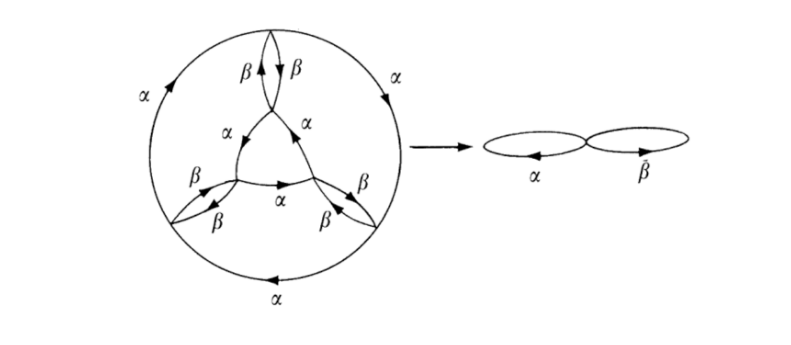
\includegraphics[width=3in]{SixFoldCover.png}
\end{center}
\begin{enumerate}[(a)]
\item Use Proposition~1.32 and Proposition~1.39 to deduce the size of the group $G(\tilde{X})$ of deck transformations. Use the symmetries of $\tilde{X}$ to identify the group $G(\tilde{X})$.
\item Alter $\tilde{X}$ by reversing the direction of the three $\alpha$ arrows on the inner circle only. What is the size of the group $G(\tilde{X})$ of deck transformations? What is the group $G(\tilde{X})$?
\end{enumerate}

\begin{proof}
By proposition 1.32 we have that the index of $p_*(\pi_1(\tilde{X},\tilde{x_0})$ in $\pi_1(X,x_0)$ is 6.  Note that the only two groups of order 6 up to isomorphism are $D_3\cong S_3$ and $\Z_6$.   Let's take a look at our 6 fold cover:
\vspace*{5cm}\\
We see that this has the presentation $H\cong\langle \alpha^3,\beta^2,(\alpha \beta)^2,\beta \alpha^3 \beta,\alpha^2\beta^2\alpha,\alpha \beta^2 \alpha^2,\alpha \beta^2\alpha^2,(\beta\alpha)^2\rangle$.  It's not hard to see that $N(H)\cong\pi_1(X,x_0)$ since we have $\alpha H \alpha^{-1} =H$ and $\beta H \beta^{-1}$ by searching a bit for elements of $H$ that commute with $\alpha$ and $\beta$. We then have
\begin{align*}
G(\tilde{X})\cong N(H)/H &\cong \langle \alpha,\beta \rangle / H\\
&\cong \langle \alpha, \beta ~\vert~ \alpha^3,\beta^2,\alpha \beta \alpha \beta \rangle\\
&\cong D_3 \cong S_3.
\end{align*}

Next, when we switch the arrows we get the following 6 fold cover:
\vspace*{5cm}\\
We see that this has the presentation $H\cong \langle \alpha^3,\beta^2,\alpha \beta \alpha^{-1}\beta^{-1},\beta \alpha^3 \beta, alpha^2 \beta^2 \alpha, \alpha \beta^2 \alpha^2, \beta \alpha \beta \alpha^2 \rangle$. Again, we find that $N(H)\cong \pi_1(X,x_0)$.  With that, we get
\begin{align*}
G(\tilde{X}) \cong N(H)/H &\cong \langle \alpha,\beta \rangle / H\\
&\cong \alpha^3,\beta^2,\alpha\beta \alpha^{-1}\beta^{-1} \rangle\\
&\cong \Z_6.
\end{align*}
\end{proof}

\vspace*{1cm}








\end{document}



